\chapter{Local da realização das atividades}
As atividades realizadas durante o período do estágio foram feitas no Núcleo de Sistemas Eletrônicos Embarcados (NSEE), laboratório localizado no Instituto Mauá de Tecnologia (IMT). Este capítulo terá uma breve descrição sobre o NSEE e o IMT.
% ---

\section{O Instituto Mauá de Tecnologia (IMT)}
Fundado em 11 de dezembro de 1961, o Instituto Mauá de Tecnologia (IMT) é uma entidade privada, sem fins lucrativos, e dedicada ao ensino e à pesquisa científica e tecnológica, com a finalidade de formar recursos humanos altamente qualificados para a contribuição do desenvolvimento do País.\cite{InstitutodeEngenharia:Online}

O IMT, com campi em São Paulo e São Caetano do Sul (Figura \ref{IMT}), mantém duas unidades: Centro Universitário e Centro de Pesquisas. O Centro Universitário oferece cursos de graduação em Administração, Design e Engenharia. Na pós-graduação, são oferecidos cursos de aperfeiçoamento, especialização e MBA nas áreas de Administração, Gestão e Engenharia e é desenvolvido programa de Mestrado em processos químicos e bioquímicos. O Centro de Pesquisas, há mais de 45 anos, desenvolve tecnologia para atendimento das necessidades da indústria.\cite{Alunos:Online}


\begin{figure}[!htb]
	\centering
	\caption{Vista aérea do \textit{Campus} do IMT de São Caetano do Sul.}
	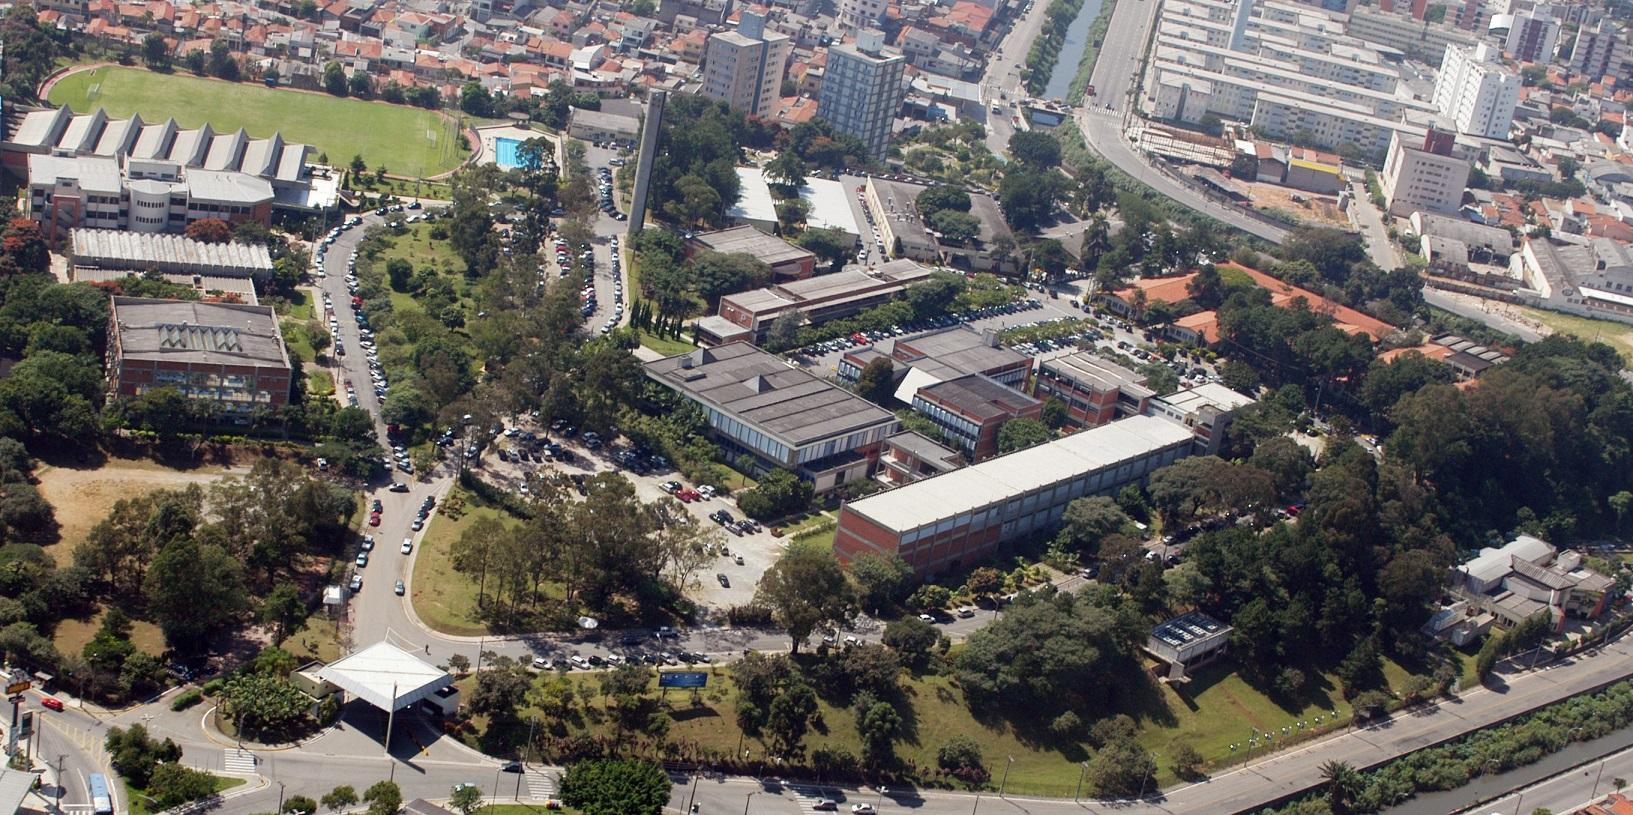
\includegraphics[scale = 1]{Imagens/Campus_IMT_foto_aerea.jpg}
	
	Fonte: Site do Wikimedia.\let\thefootnote\relax\footnotemark[1]
		
	\label{IMT}
\end{figure}

\let\thefootnote\relax\footnotetext[1]{Figura retirada da URL \url{https://upload.wikimedia.org/wikipedia/commons/3/3e/Campus_foto_a\%C3\%A9rea.jpgl}. Acesso em: 7 out. 2015}


% ---

% ---
\section{O Núcleo de Sistemas Eletrônicos Embarcados (NSEE)}
Para saber um pouco mais sobre o novo laboratório Núcleo de Sistemas Eletrônicos Embarcados (NSEE), antes de tudo é preciso entender que sistemas embarcados são uma classe de sistemas digitais voltados e desenvolvidos para aplicações específicas, apresentando, frequentemente, restrições de processamento em tempo real. Apesar da complexidade do tema, esse tipo de tecnologia já faz parte de objetos do nosso cotidiano, como GPS e telefones celulares e vem sendo cada dia mais utilizada nas áreas automotiva, espacial, industrial e de entretenimento.

Criado no início do ano de 2010, o Núcleo coordenado pelo professor Vanderlei Cunha Parro, além de ter como objetivo o estudo e o desenvolvimento desse tipo de sistema, também possui outros temas de interesse, como aplicações em processamento de sinais, controle digital e experimentos aeroespaciais.\cite{NovoLaboratorioNSEE:Online}

O laboratório possui vários computadores e um amplo espaço para realizações de diversos projetos. Possui também componentes e equipamentos eletrônicos que auxiliam nas diversas tarefas, como fontes de alimentação, multímetro e osciloscópio. Há também o almoxarifado de componentes e equipamentos eletrônicos no piso superior que oferece um suporte a mais ao NSEE e, consequentemente, aos projetos realizados no laboratório. 

O ambiente do NSEE também favorece o estudo e aprendizado. Os alunos e pesquisadores procuram sempre ajudar um ao outro em suas dificuldades fazendo com que todos possam crescer juntos.

% ---